% \section{A Conflict Graph-Based Approach}\label{sec:graph-algorithms}

% For the minimum inconsistency measure $\mininconsistency$ and the problematic measure $\problematic$, we model our problem using the conflict graph and control the sensitivity using graph projection techniques~\cite{kasiviswanathan2013analyzing, blocki2013differentially, day2016publishing} and for the $\repair$ measure, we come up with an approximate DP vertex cover size algorithm. 


\section{Leveraging Graph Projection for \mininconsistency~ and \problematic}\label{sec:graph-algorithms-graphproj}

% \xh{Suggested outline:
% \begin{itemize}
%     \item Intro paragraph: recap the two measures and their high sensitivity; describe high-level ideas of our approach from prior work on graphs and their issues still; describe a high-level idea of our approach deals with their problem (which is the core contribution); summarize the organization structure of this section and mention that we use \mininconsistency to illustrate the algorithms and \problematic is similar. [the current intro is in a similar flow as this, but add the structure and the note]  
%     \item Sec 4.1 DC Oblivious DP Algorithm:  summarize the end-to-end algorithm with an algorithm box (Algorithm 1) that includes 3 main steps: (1) Exponential mechanism (EM) for optimal theta; (2) graph projection; (3) Noise addition with Laplace mechanism (for EM and graph projection, we can have a separate algorithm box for each, Algorithm 2 and Algorithm 3). This serves as a baseline algorithm that makes no use of the knowledge of DC in the original database, but only the conflict graph. All the contents here are adapted from prior work. 
%     \begin{itemize}
%         \item Sec 4.1.1 Project Projection for Theta-bounded Graph (algorithm description and sensitivity of for edge count)
%         \item Sec 4.1.2 Exponential Mechanism for Theta (algorithm description, score function, and sensitivity)
%         \item Sec 4.1.3 Privacy and Utility Analysis: here we can highlight the utility issues of this algorithm
%     \end{itemize}
%     \item Sec 4.2. DC-aware DP Algorithm: how to improve the candidate set using DCs/FDs;  The algorihtm box here can include the details of current Algorithm 2 (theta candidate section) and then run Algorithm 1 which takes the updated Theta as input. 
%     \begin{itemize}
%         \item Sec 4.2.1 Candidate Curation 
%         \item Sec 4.2.2 Privacy analysis 
%     \end{itemize}
% \end{itemize}
% }

% \ag{We cannot just start referring to the problem as a problem over the conflict graph. We need to say in section 3 that we assume that we can compute the conflict graph privately and from that point, we compute all measures on that.}

% $\mininconsistency$ and $\problematic$ measures essentially pertain to the total number of edges ($|E|$) and the total number of nodes with positive degrees, respectively, in the conflict graph $\graph(V, E)$. We analyze that computing these measures directly using the Laplace mechanism entails high sensitivity ($\propto |V|$) as shown in ~\cref{prop:sens_mininconsistency_noproj}.

As we saw in Proposition~\ref{prop:sens_mininconsistency_problematic_naive}\xh{not great way to start a section}, the sensitivity for $\mininconsistency$ and $\problematic$ could be very high \xh{be specific how high it is. note that drast and MC measures also have high sensitivity, why we do not consider them for further algorithmd evelopment}. We observe that this high sensitivity stems from the fact that adding or removing one row could potentially affect all other connected rows. Therefore, it is of utmost importance to bound these connections for accurate private estimation.  In our work, we take a natural graphical approach and model the violations and their relations with other tuples in the datasets using conflict graphs. We illustrate this in Example~\ref{example:running_example}. 

\xh{This intro is quite long. We can break it into a shorter intro and a new subsection on "Graph Project Approach" or something like that. }

\begin{example}
     Consider a dataset that stores information about occupation and income as shown in Figure~\ref{fig:db_to_graph}. Assume an FD constraint $\sigma$ between attributes country and capital that says that the capital has to be similar if the country is the same $\sigma: \neg (t_i[country]=t_j[country] \land t_i[capital] \neq t_j[capital])$. Assume the dataset has 3 rows (white color) and a neighboring dataset has an extra row (grey color). As shown in the right side of Figure~\ref{fig:db_to_graph}, the dataset with 4 rows can be converted to a conflict graph with the nodes corresponding to each tuple and edges referring to conflicts between them. The $\mininconsistency$ measure that computes the size of the set of all minimally inconsistent subsets $|MI_\constraintset(D)|$ (the number of edges in the graph) for this dataset has a sensitivity equal to the size of the dataset (in this case, 3) as adding a violating row violates all other rows.
     \label{example:running_example}
\end{example}


% \begin{tikzpicture}

% % Table
% \matrix[matrix of nodes,
%         nodes={draw, minimum width=2cm, minimum height=1cm, align=center},
%         row sep=0.5cm, column sep=0.5cm] (table) {
%     ID & Country & Capital \\
%     1 & Canada & Ottawa \\
%     2 & Canada & Ottawa \\
%     3 & Canada & Ottawa \\
%     4 & USA & Ottawa \\
% };

% % Graph
% \node[draw, circle, minimum size=1cm] at (6cm, 1cm) (node1) {1};
% \node[draw, circle, minimum size=1cm] at (7cm, 1cm) (node2) {2};
% \node[draw, circle, minimum size=1cm] at (6.5cm, 0cm) (node3) {3};
% \node[draw, circle, minimum size=1cm] at (6.5cm, 1cm) (node4) {4};

% \draw (node1) -- (node2);
% \draw (node1) -- (node4);
% \draw (node3) -- (node4);

% % Arrow
% \draw[->] (table-4-3) -- (node4);

% \end{tikzpicture}




\begin{figure}
    \centering
    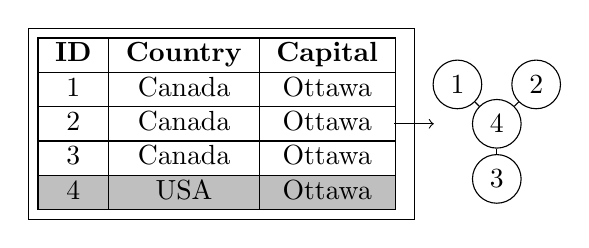
\begin{tikzpicture}
    % Define the table
    \node[draw, align=center] (table) at (1.5,0) {
        \begin{tabular}{|c|c|c|}
            \hline
            \textbf{ID} & \textbf{Country} & \textbf{Capital} \\
            \hline
            1 & Canada & Ottawa \\
            \hline
            2 & Canada & Ottawa \\
            \hline
            3 & Canada & Ottawa \\
            \hline
             \rowcolor{lightgray}
            4 & USA & Ottawa \\
            \hline
        \end{tabular}
    };

    % Define the graph
    
    \node[draw, circle] (node1) at (4.5,0.5) {1};
    \node[draw, circle] (node2) at (5.5,0.5) {2};
    \node[draw, circle] (node3) at (5,-0.7) {3};
    \node[draw, circle] (node4) at (5,0) {4};
    \draw (node1) -- (node4);
    \draw (node2) -- (node4);
    \draw (node3) -- (node4);
    
    % Draw the arrow
    % \draw[->] (table.east) -- (node4.west);
    \draw[->] (3.7, 0) -- (4.2, 0);
\end{tikzpicture}
   \vspace{0.2cm} % Add space below the figure
    % \includegraphics[width=\linewidth]{images/database_to_graph.jpg}
    \caption{Toy example dataset to show a worst-case analysis. An additional row may violate all other rows in the dataset (left). Easier analysis can be done by instead converting the dataset into its corresponding conflict graph (right).
    }
    \label{fig:db_to_graph}
    % Image link: https://docs.google.com/drawings/d/1ibadfqHlWPfEwiOApukretrSKzGyi9w6-pv5OX8Y3sI/edit?usp=sharing
\end{figure}


Based on this transformation of the input dataset $D$ and its constraints $\constraintset$ to a conflict graph $\graph$, we slightly modify our problem statement to these inconsistency measures $I(\graph, \constraintset)$ on the conflict graph $\graph$ to an equivalent formulation based on~\cref{prop:graph-defs}.

\begin{problem}[Inconsistency measures on conflict graph]\label{prob:measure_graph}
Consider the same setup as Problem~\ref{prob:measure_dataset} along with the conflict graph $\graph$. We would like to obtain an $\epsilon$-DP algorithm $M(\graph, \constraintset, \epsilon)$ for an inconsistency measures $I(\graph, \constraintset)$ such that with high probability, $|M(\graph, \constraintset, \epsilon) - I(\graph, \constraintset)|$ is bounded with a small error.
\end{problem}

The new problem statement makes two modifications. First, the input translates from the input dataset $D$ to its corresponding conflict graph $\graph$. Second, the DP definition changes to node-DP, where a neighbouring graph can be obtained by adding or removing a node. Using this setup, we can now control the connectivity amongst tuples using their corresponding nodes' degree in the conflict graph $\graph$. We do so by leveraging the graph projection using edge addition algorithm~\cite{day2016publishing}. Precisely, to accurately estimate these measures with DP, we bound the degree of every vertex in the graph to a new value $\theta$, calculate the new sensitivity on the bounded graph, and add Laplace noise proportional to the new sensitivity estimate. However, we observe that an important decision in this process is to choose the maximum degree bound value of $\theta$. We find that the optimum $\theta$ value heavily depends on the density of the graph, and the favored technique of exponential mechanism~\cite{mcsherry2007mechanism} used by prior work~\cite{day2016publishing} fails due to a large number of candidates and high sensitivity of the quality function. Therefore, to improve our algorithm, we develop an enhanced search process that smartly uses denial constraints in the constraint set $\constraintset$. In this section, we first show an overview of our algorithm that uses graph projection to bound the sensitivity on conflict graphs. Then, we improve the algorithm using some optimization techniques that enhance the search process of the exponential mechanism using two improvements based on the constraints available to us in the constraint set $\constraintset$.   

The rest of the section is organized into two subsections. In the first subsection, we introduce our algorithm, detail the specifics of the graph projection and parameter selection techniques, and its privacy and utility analysis. Using the utility analysis, we identify that our algorithm depends heavily on the parameter selection process. In the second subsection, we illustrate two optimization techniques based on the constraint set that can significantly improve the parameter selection process and, thereby, the algorithm's utility. 


% In this section, we illustrate our algorithm using the minimum inconsistency $\mininconsistency$ measure that concerns the total number of edges in the graph. The problematic $\problematic$ measure that involves the total number of positive degree nodes in the graph has a similar algorithm. First in \cref{sec:dc_oblivious_algo}, we summarize the end-to-end algorithm for computing these measures and analyze both its privacy and utility analysis. We highlight that the candidate set $\Theta$ plays a crucial role in the utility of the algorithm. In section \cref{sec:dc_aware_algo}, we improve our algorithm by curation candidate set.

\subsection{Overview}\label{sec:dc_oblivious_algo}

Our algorithm for computing the $\mininconsistency$ and $\problematic$ using graph projection involves four main steps as shown in Algorithm~\ref{algo:dc_oblivious} that takes as input the dataset $D$, constraint set $\constraintset$, a candidate set $\Theta$ for prospective bounds, and privacy budgets $\epsilon_1$ and $\epsilon_2$. First, in line 1, we start by computing the conflict graph $\graph$ generated from the input dataset $D$ and constraint set $\constraintset$. Graph $\graph$ contains nodes for each tuple in the dataset and edges for all violations between tuples. In Line 2, we compute a value of $\theta^*$ from the candidate set $\Theta$ using the exponential mechanism and part of the privacy budget $\epsilon_1$ as described in Section~\ref{sec:expo_mech}. Next in line 3, we compute a bounded graph $\mathcal{G}_{\theta^*}$ using the graph projection using edge addition algorithm~\cite{day2016publishing}, we compute a compute bounded graph $\pi_{\theta^*}^\Lambda$ such that each node in the new graph has a degree no greater than $\theta^*$ as detailed in Section~\ref{sec:prelim}. Finally, in line 4, we compute the measure (either the number of edges for $\mininconsistency$ or the number of positive degree nodes for $\problematic$) on $\mathcal{G}_{\theta^*}$ by adding Laplace noise using the other half of the privacy budget $\epsilon_2$. 


\begin{algorithm}
\caption{Algorithm overview}
\label{algo:dc_oblivious}
    \KwData{Dataset $D$, Constraint set $\constraintset$, Candidate set $\Theta$, Privacy Budgets $\epsilon_1$ and $\epsilon_2$}
    \KwResult{Inconsistency measure $\mininconsistency$ or $\problematic$}
    Compute conflict graph $\graph$ using dataset $D$ and $\constraintset$\\
    Find optimal theta $\theta^*$ from $\Theta$ using Exponential mechanism using budget $\epsilon_1$\ \redtext{(Algorithm~\ref{algo:expo_mech})}\;
    Compute $\theta^*$-bounded graph $\mathcal{G}_{\theta^*}$ \redtext{(Edge addition algorithm~\cite{day2016publishing})}\;
    Compute measure on $\mathcal{G}_{\theta^*}$ by adding Laplace noise using budget $\epsilon_2$

\end{algorithm}

The inconsistency measures $\mininconsistency$ and $\problematic$ can be directly computed on the bounded graph. For the $\mininconsistency$, we compute the total number of edges $\pi_\theta(\mathcal{G})$. The sensitivity analysis of $\mininconsistency$ on $\pi_\theta(\mathcal{G})$ is detailed in \cref{lemma:sens_mininconsistency}.

\begin{lemma}
    The sensitivity of $\mininconsistency(\pi_\theta(\mathcal{G}))$ is $\theta$, where $\pi_\theta$ is the edge addition algorithm with the user input $\theta$.
        % $$\| \mininconsistency(\pi_{\theta}^\Lambda(\mathcal{G})) - \mininconsistency(\pi_{\theta}^\Lambda(\mathcal{G}^\prime)) \| \leq \theta$$ 
    \label{lemma:sens_mininconsistency}
\end{lemma}

\ifpaper
The lemma can be proved by analyzing the changes made to the degree of each node in the graph by adding one edge at a time. The stable ordering of the edges allows us to keep track of the edges for two neighbouring graphs. Due to space constraints, we defer the proof to the full paper.  
\else
\proof
Let's assume without loss of generality that
$\mathcal{G}^{\prime}=\left(V^{\prime}, E^{\prime}\right)$ has an additional node $v^{+}$compared to $\mathcal{G}=$ $(V, E)$, i.e., $V^{\prime}=V \cup\left\{v^{+}\right\}, E^{\prime}=E \cup E^{+}$, and $E^{+}$is the set of all edges incident to $v^{+}$in $\mathcal{G}^{\prime}$. Let $\Lambda^{\prime}$ be the stable orderings for constructing $\pi_\theta\left(\mathcal{G}^{\prime}\right)$, and $t$ be the number of edges added to $\pi_\theta\left(\mathcal{G}^{\prime}\right)$ that are incident to $v^{+}$. Clearly, $t \leq \theta$ because of the $\theta$-bounded algorithm. Let $e_{\ell_1}^{\prime}, \ldots, e_{\ell_t}^{\prime}$ denote these $t$ edges in their order in $\Lambda^{\prime}$. Let $\Lambda_0$ be the sequence obtained by removing from $\Lambda^{\prime}$ all edges incident to $v^{+}$, and $\Lambda_k$, for $1 \leq k \leq t$, be the sequence obtained by removing from $\Lambda^{\prime}$ all edges that both are incident to $v^{+}$and come after $e_{\ell_k}^{\prime}$ in $\Lambda^{\prime}$. Let $\pi_\theta^{\Lambda_k}\left(\mathcal{G}^{\prime}\right)$, for $0 \leq k \leq t$, be the graph reconstructed by trying to add edges in $\Lambda_k$ one by one on nodes in $\mathcal{G}^{\prime}$, and $\lambda_k$ be the sequence of edges from $\Lambda_k$ that are actually added in the process. Thus $\lambda_k$ uniquely determines $\pi_\theta^{\Lambda_k}\left(\mathcal{G}^{\prime}\right)$; we abuse the notation and use $\lambda_k$ to also denote $\pi_\theta^{\Lambda_k}\left(\mathcal{G}^{\prime}\right)$. We have $\lambda_0=\pi_\theta(\mathcal{G})$, and $\lambda_t=\pi_\theta\left(\mathcal{G}^{\prime}\right)$.

In the rest of the proof, we show that $\forall k$ such that $1 \leq k \leq t$, at most 1 edge will differ between $\lambda_k$ and $\lambda_{k-1}$. This will prove the lemma because there are at most $t$ (upper bounded by $\theta$) edges that are different between $\lambda_t$ and $\lambda_0$.

To prove that any two consecutive sequences differ by at most 1 edge, let's first consider how the sequence $\lambda_k$ differs from $\lambda_{k-1}$. Recall that by construction, $\Lambda_k$ contains one extra edge in addition to $\Lambda_{k-1}$ and that this edge is also incident to $v^*$. Let that additional differing edge be $e_{\ell_k}^\prime = (u_j, v^+)$. In the process of creating the graph $\pi_\theta^{\Lambda_k}(\mathcal{G}^{\prime})$, each edge will need a decision of either getting added or not. The decisions for all edges coming before $e_{\ell_k}^{\prime}$ in $\Lambda^{\prime}$ must be the same in both $\lambda_k$ and $\lambda_{k-1}$. Similarly, after $e_{\ell_k}^{\prime}$, the edges in $\Lambda_k$ and $\Lambda_{k-1}$ are exactly the same. However, the decisions for including the edges after $e_{\ell_k}^{\prime}$ may or may not be the same. Assuming that there are a total of $s \geq 1$ different decisions, we will observe how the additional edge $e_{\ell_k}^{\prime}$ makes a difference in decisions. 


When $s=1$, the only different decision must be regarding differing edge $e_{\ell_k}^\prime = (u_j, v^+)$ and that must be including that edge in the total number of edges for $\lambda_k$. Also note that due to this addition, the degree of $u_j$ gets added by 1 which did not happen for $\lambda_{k-1}$. When $s>1$, the second different decision must be regarding an edge incident to $u_j$ and that is because degree of $u_j$ has reached $\theta$, and the last one of these, denoted by $(u_j, u_{i \theta})$ which was added in $\lambda_{k-1}$, cannot be added in $\lambda_k$. In this scenario, $u_j$ has the same degree (i.e., $\theta$ ) in both $\lambda_k$ and $\lambda_{k-1}$. Now if $s$ is exactly equal to 2, then the second different decision must be not adding the edge $(u_j, u_{i \theta})$ to $\lambda_k$. Again, note here that as $(u_j, u_{i \theta})$ was not added in $\lambda_k$ but was added in $\lambda_{k-1}$, there is still space for one another edge of $u_{i \theta}$. If $s>2$, then the third difference must be the addition of an edge incident to $u_{i \theta}$ in $\lambda_k$. This process goes on for each different decision in $\lambda_k$ and $\lambda_{k-1}$. Since the total number of different decisions $s$ is finite, this sequence of reasoning will stop with a difference of at most 1 in the total number of the edges between $\lambda_{k-1}$ and $\lambda_k$.
\qed
\fi

For the $\problematic$ measure, that is the total number of nodes in the graph that have a positive degree, we compute the number of nodes in the $\pi_\theta(\mathcal{G})$ that have degree 0 and subtract it from the total nodes in the graph. The sensitivity analysis of $\problematic$ is given by ~\cref{lemma:sens_problematic}. 

\begin{lemma}
    The sensitivity of $\problematic(\pi_\theta(\mathcal{G}))$ is $\theta$, where $\pi_\theta$ is the edge addition algorithm with user input $\theta$.
        % $$\| \problematic(\pi_\theta(\mathcal{G})) - \problematic(\pi_\theta(\mathcal{G}^\prime)) \| \leq \theta$$ 
    \label{lemma:sens_problematic}
\end{lemma}

\proof
Assume, in the worst case, the graph $\mathcal{G}$ is a star graph with $n$ nodes such that there exists an internal node that is connected to all other $n-1$ nodes. In this scenario, there are no nodes that have 0 degrees, and the $\problematic$ measure $= n-0 = 0$. If the neighbouring graph $\mathcal{G}^\prime$ differs on the internal node, all edges of the graph are removed are the $\problematic = n$. The edge addition algorithm $\pi_\theta$ would play a minimal role here as $\theta$ could be equal to $n$.
\qed



\subsubsection{Parameter selection}\label{sec:expo_mech}

The value of $\theta$ is a user-defined hyperparameter in the edge addition algorithm that plays a crucial role in estimating the inconsistency measures. However, unfortunately, the optimal value of $\theta$ may vary significantly across datasets. Higher values of $\theta$ in the edge addition algorithm $\pi_\theta$ may preserve more edges of the original graph but introduce higher error from the Laplace noise. In contrast, smaller values of $\theta$ may have lower Laplace noise error but truncate a significant number of edges, thereby introducing substantial error as well as shown later in Example~\ref{example:parameter_selection}. Therefore, accurately estimating both measures necessitates selecting an appropriate value for $\theta$.

A popular algorithm for this purpose of choosing hyperparameters like $\theta$ is the exponential mechanism~\cite{mcsherry2007mechanism} as shown in Algorithm~\ref{algo:expo_mech}. Given a candidate set $\Theta$ with max value $\theta_{max}$ and a quality function $q(\mathcal{G}, \theta) \in \mathbb{R}$ and corresponding scores for each candidate, exponential mechanism picks a candidate $\theta^* \in \Theta$ that has the highest score with high probability.

\begin{algorithm}
\caption{Parameter selection algorithm}
\label{algo:expo_mech}
    \KwData{Graph $\mathcal{G} (V,E)$, Candidate set $\Theta$, Quality function $q$, Privacy budget $\epsilon_1, \epsilon_2$ }
    \KwResult{Candidate $\theta^*$}
    Find max value in $\Theta$ as $\theta_{max}$ \;
    For each candidate $\theta_i \in \Theta$, compute $q(\mathcal{G}, \theta_i, \theta_{max},  \epsilon_2)$ \;
    Pick $\theta^*$ with prob $\propto \exp( \frac{\epsilon_1 q(\mathcal{G}, \theta_i, \theta_{max}, \epsilon_2)}{2\Delta_q})$\;
    return $\theta^*$\;

\end{algorithm}

The quality function that we choose for computing the measures includes two terms. The first term $e_{measure}$  captures the quality of the measure, and the second term $e_{privacy}$ captures the error from the noise added due to privacy. For the minimum inconsistency $\mininconsistency$ measure that computes the $e_{measure}(\mathcal{G}, \theta_{max}, \theta) = |\mathcal{G}_{\theta_{max}}.E - \mathcal{G}_\theta.E|$, this term computes the number of edges that are truncated due to the projection algorithm as compared to the truncation using $\theta_{max}$. For the problematic $\problematic$ measure that computes the number of positive degree vertices, $e_{measure}(\mathcal{G}, \theta_{max}, \theta) = d_0^{\mathcal{G}_{\theta_{max}}} - d_0^{\mathcal{G}^\prime}$, where $d^\mathcal{G}_0$ is a function that counts the number of vertices in $\mathcal{G}$ with $0$ degree. 
The second term for both measures is equal to the standard deviation of the Laplace noise based on the sensitivity of these measures. Precisely, this second term is common for both the measures proportional to $e_{privacy} (\theta, \epsilon) =  \sqrt{2}\frac{\theta}{\epsilon}$ as the sensitivity for both the measures is equal to the same value $\theta$ as per our analysis in  \cref{lemma:sens_mininconsistency} and \cref{lemma:sens_problematic}. Therefore, the final quality function for the exponential mechanism is 
\begin{equation}~\label{eq:quality_function}
    q(\mathcal{G}, \theta, \theta_{max}, \epsilon) = - e_{measure}(\mathcal{G}, \theta_{max}, \theta) - e_{privacy} (\theta, \epsilon)
\end{equation}
The two terms of the quality function in equation~\ref{eq:quality_function} balance the error generated from measure computation and noise addition. If a candidate $\theta_i$ is too low, then the error from the privacy term $e_{privacy}$ would be low, but the error from the measure $e_{measure}$ would be high and vice versa if $\theta_i$ is too high. We illustrate this using an example. 

\begin{example}~\label{example:quality_function}
    Consider the same graph as Example~\ref{example:running_example} and a candidate set $\Theta = [1, 2, 3]$ to compute the $\mininconsistency$ measure (number of edges) with $\epsilon=1$. For the first candidate $\theta_1 = 1$, as node 4 has degree 3, the edge addition algorithm would truncate 2 edges, for $\theta_2 = 2$, 1 edge would be truncated and for $\theta_3 = 3$, no edges would be truncated. We can, therefore, compute each term of the quality function for each $\theta$ given in Table~\ref{tab:example_quality_function}.  
    \begin{table}[]
        \centering
        \begin{tabular}{|c|c|c|c|}
             \hline
             $\theta$ & $e_{measure}$ & $e_{privacy}$ & q  \\
             \hline
             1 & 2 & $\sqrt{2}$ & $-2 - \sqrt{2}$\\
             2 & 1 & $\sqrt{2} * 2$ &  $-1 - 2\sqrt{2}$\\
             3 & 0 & $\sqrt{2} * 3$ & $-3\sqrt{2}$\\
             \hline
        \end{tabular}
        \caption{Quality function computation}
        \label{tab:example_quality_function}
    \end{table}
    For this example, we see that $\theta_1$ has the best quality even if it truncates the most number of edges as the error from privacy overwhelms the error from measure computation. 
\end{example}

In Lemma~\ref{lemma:sens_quality}, we show the sensitivity computation for the quality function for the $\mininconsistency$ measure. The $\problematic$ measure has a similar analysis. 

\begin{lemma}
    For any two neighbouring graphs $\mathcal{G}$ and $\mathcal{G}^\prime$, the sensitivity of the quality function $q(\mathcal{G}, \theta_i)$ equals $\theta_{max}$,
    % $$\|q(\mathcal{G}, \theta_i) - q(\mathcal{G}^\prime, \theta_i)\| \leq \theta_{max}$$
    where $\theta_{max}$ is the maximum theta value over all candidate values $\theta_i \in \Theta$.
\end{lemma}\label{lemma:sens_quality}
\begin{proof}
    \begin{equation*}
        \begin{split}
            \|q(\mathcal{G}, \theta_i) - q(\mathcal{G}^\prime, \theta_i)\| &\leq -|\mathcal{G}_{\theta_{max}}.E - \mathcal{G}_{\theta_i}.E| - \sqrt{2}\frac{\theta_i}{\epsilon_1} \\ &+ |\mathcal{G}'_{\theta_{max}}.E - \mathcal{G}'_{\theta_i}.E| + \sqrt{2}\frac{\theta_i}{\epsilon_1} \\
            &\leq |\mathcal{G}'_{\theta_{max}}.E - \mathcal{G}_{\theta_{max}}.E| - |\mathcal{G}'_{\theta_{i}}.E - \mathcal{G}_{\theta_{i}}.E|\\
            &\leq \theta_{max} - \theta_i \\
            &\leq \theta_{max}            
        \end{split}
    \end{equation*}
\end{proof}

\subsubsection{Privacy and utility analysis}\label{sec:dc_oblivious_privay_util}

The privacy analysis of \cref{algo:dc_oblivious} depends on the privacy budget spent for the exponential mechanism and the final measure calculation as shown in Theorem~\ref{thm:privacy_proof_dc_oblivious}.

\begin{theorem}\label{thm:privacy_proof_dc_oblivious}
    \cref{algo:dc_oblivious} satisfies $\epsilon_1 + \epsilon_2$-node DP.
\end{theorem}
\begin{proof}
    In \cref{algo:dc_oblivious}, Line 1 uses the exponential mechanism with $\epsilon_1$ to calculate $\theta^*$. This theta value is then used to compute the bounded graph, and finally, the inconsistency measure value is released with Laplace noise of $\epsilon_2$. Therefore, using composition properties of DP, \cref{algo:dc_oblivious} satisfies $\epsilon_1 + \epsilon_2$-node DP.
\end{proof}

For the utility analysis of \cref{algo:dc_oblivious}, we analyze the utility of the exponential mechanism that outputs the best value of $\theta^*$. As per Theorem~\ref{thm:utility_expo}, the exponential mechanism allows us to privately select an object $\theta$ from a set of objects $\Theta$ with a score comparable to the best score $OPT$ in $\Theta$ with an error that depends on the sensitivity, privacy budget $\epsilon$ and the total number of candidates $|\Theta|$. Theorem~\ref{thm:utility_proof} shows the utility analysis of inconsistency measures using Algorithm~\ref{algo:dc_oblivious}. 


\begin{theorem}\label{thm:utility_proof}
Let $\mathcal{G}(V, E)$ be a private graph, and $OPT(\mathcal{G})=\max _{\theta \in \Theta} q(\mathcal{G}, \theta, |V|, \epsilon_1, \epsilon_2)$ be the quality attained by the best object $\theta$ with respect to the dataset $\mathcal{G}$ due to Algorithm~\ref{algo:dc_oblivious}, $M(\mathcal{G})$. If the set of objects that achieve the $OPT(\mathcal{G})$, $\Theta^*=\{\theta \in \Theta: q(\mathcal{G}, \theta, |V|, \epsilon_1, \epsilon_2)=OPT(\mathcal{G})\}$ has size $|\Theta^*| \geq 1$. Then
$$ \Pr \left[q(\mathcal{G}, M(\mathcal{G}), |V|, \epsilon_1, \epsilon_2) \leq OPT (\mathcal{G}) - \frac{2|V|}{\epsilon_1} (\ln |\Theta| + t) \right] \leq \exp(-t)$$,
where $\epsilon_1$ and $\epsilon_2$ are the privacy budgets for the exponential mechanism and measure calculation respectively, $q$ is the quality function that measures the quality of the minimum inconsistency measure $\mininconsistency$.
\end{theorem}


\proof

The result can be obtained by plugging in the sensitivity value of the utility function $\Delta_q = \theta_{max} = |V| $ to \cref{thm:utility_expo}. 

% \begin{equation*}
%     \begin{split}
%         \Pr\left[q(\mathcal{G}, M(\mathcal{G}), |V|, \epsilon_1, \epsilon_2) \leq OPT (\mathcal{G}) - \frac{2|V|}{\epsilon_1} (\ln |\Theta| + t) \right] \leq \exp(-t)
%     \end{split}
% \end{equation*}
\qed

According to Theorem~\ref{thm:utility_proof}, the utility of Algorithm~\ref{algo:dc_oblivious} is directly proportional to the number of candidates $|\Theta|$ and the sensitivity of the quality function equivalent to number of nodes in the graph $|V|$. However, in practice, these values can be extremely large depending on the density of the graph, which is an artifact of the number of conflicts in the dataset. Luckily, for our use case, these conflicts arise from the denial constraints in the constraint set $\constraintset$ that are available to us. In the next section, we show how we can make use of these constraints to improve the utility of our algorithm by truncating candidates in the set $\Theta$.

\subsection{Optimized Parameter Selection}\label{sec:dc_aware}

Our developed strategy to improve the parameter selection includes two optimization techniques. The overarching idea behind these optimizations is to gradually truncate large candidates from the candidate set $\Theta$ based on the density of the graph. For example, we observe that the Stock dataset~\cite{oleh_onyshchak_2020} has a sparse conflict graph, and its optimum degree for graph projection is in the range of $10^0-10^1$. In contrast, the graph for the Adult dataset sample~\cite{misc_adult_2} is extraordinarily dense and has an optimum degree $\theta$ greater than $10^3$, close to the sampled data size. 
Removing unneeded large candidates, especially those greater than the true maximum degree of the graph, can help the high sensitivity issue of the quality function and improve our chances of choosing a better bound. 

Our first optimization estimates an upper bound for the true maximum degree of the conflict graph and removes candidates larger than this upper bound from the initial candidate set. The second optimization is a hierarchical exponential mechanism that utilizes two steps of exponential mechanisms. The first output, $\theta^1$, is used to truncate $\Theta$ further by removing candidates larger than $\theta^1$ from the set, and the second output is chosen as the final candidate $\theta^*$. In the rest of this section, we dive deeper into the details of these optimizations and discuss their privacy analysis. 

% In Algorithm~\ref{algo:dc_aware}, we show the improved version of our algorithm. We truncate values in the candidate set $\Theta$ in a two-step process. In lines 1-2, we first use the constraints in $\constraintset$ that are FDs to find an upper bound of the maximum degree of vertices in the graph denoted by $\theta_{bound}$ and remove candidates larger than this threshold. Second, in line 3, we use a two-step exponential mechanism to choose a value of $\theta^*$. The output of the first step, $\theta^1$, is used to truncate $\Theta$ further by removing candidates larger than $\theta^1$. The output of the second step is chosen as the final candidate $\theta^*$. The rest of the algorithm lines 4-5 is similar to the DC oblivious counterpart of the algorithm, where we project the graph and compute the inconsistency measures. In the rest of the section, we dive deeper into the details of this algorithm and discuss the privacy analysis. 


\paratitle{Estimating the degree upper bound using FDs} \label{sec:dc_aware_ub}
%The maximum degree of a conflict graph $\graph$ is governed by the total number of conflicts and its density properties. As discussed earlier at the start of the section, the densities of different real-world conflict graphs vary immensely. In our use case, as the datasets that give rise to these conflict graphs are private, the density properties of the conflict graphs are unknown. 
Given a conflict graph $\graphsimple(V,E)$, we use $\degree(\graphsimple, v)$ to denote the degree of the node $v\in V$ in $\graphsimple$ and $\degree_{\max}(\graphsimple) = \max_{v\in V} \degree(\graphsimple, v)$ to denote the maximum degree in $\graphsimple$. We estimate $\degree_{\max}$ by leveraging how conflicts were formed for its corresponding dataset $D$ under $\constraintset$. 

The degree for each vertex in $\graphsimple$ can be found by going through each tuple $t$ in the database $D$ and counting the tuples that violate the $\constraintset$ jointly with $t$.
However, computing this value for each tuple is computationally expensive and highly sensitive, making it impossible to learn directly with differential privacy.  
We observe that the conflicts that arise due to functionality dependencies (FDs)  depend on the values of the left attributes in the FD. 
\begin{example}
    Consider the same setup as  Example~\ref{example:running_example}  and an FD 
$\sigma: \text{Capital}\rightarrow \text{Country}$. 
%    $\sigma : \forall t_i, t_j \dots \in D, \neg(t_i[Occupation] = t_j[Occupation] \land t_i[Income] \neq t_j[Income])$. 
We can see that the number of violations added due to the erroneous grey row is 3. This number is also one smaller than the maximum frequency of values occurring in the Capital attribute, and the most frequent value is ``Ottawa''.
\end{example}

Based on this observation, we can derive an upper bound for the maximum degree of a conflict graph if it involves only FDs, and this upper bound has a lower sensitivity. We show the upper bound in Lemma~\ref{lemma:fd_theta} for one FD first and later extend for multiple FDs.  

\begin{lemma}\label{lemma:fd_theta}
Given a database $D$ and 
a FD $\sigma: X\rightarrow Y$ as the single constraint,
where $X = \{A_1,\dots,A_k\}$ and $Y$ is a single attribute. For its respective conflict graph $\graphsimple^D_{\Sigma = \{\sigma\}}$, simplified as $\graphsimple^D_{\sigma}$, we have the maximum degree of the graph $\degree_{\max}(\graphsimple^D_{\sigma})$ upper bounded by
    \begin{equation}
     \degreebound(D,X)
    =
    \max_{\vec{a_X} \in \dom(A_1) \times \ldots \times \dom(A_k) }  \normalfont{\text{freq}}(D, \vec{a_X})-1, 
    \end{equation}    
where $\normalfont{\text{freq}}(D, \vec{a_X})$ is the frequency of values $\vec{a_X}$ occurring for the attributes $X$ in the database $D$. 
The sensitivity for $\degreebound(D,X)$ is 1. %all $\normalfont{\text{freq}}(D, a_x)$ together is 1. 
\end{lemma}

\begin{proof}
An FD violation can only happen to a tuple $t$ with other tuples $t'$ that share the same values for the attributes $X$. 
Let $\vec{a_X}^*$ be the most frequent value for $X$ in $D$, i.e., 
$$\vec{a_X}^*=\text{argmax}_{\vec{a_X} \in \dom(A_1) \times \ldots \times \dom(A_k) } \normalfont{\text{freq}}(D, \vec{a_X}).$$
In the worst case, a tuple $t$ has the most frequent value $\vec{a_X}^*$ for $X$ but has a different value in $Y$ with all the other tuples with $X=\vec{a_X}^*$. Then the number of violations involved by $t$ is $\text{freq}(D,\vec{a_X}^*)-1$.

Adding a tuple or removing a tuple to a database will change, at most, one of the frequency values by 1. Hence, the sensitivity of  the maximum frequency values is 1.
\end{proof}

Now, we will extend the analysis to multiple FDs. 
\begin{theorem}\label{theorem:fd_theta}
Given a database $D$ and a set of FDs 
$\constraintset=\{\sigma_1,\ldots,\sigma_l \}$, for its respective conflict graph $\graph$, we have the maximum degree of the graph $\degree_{\max}(\graph)$ upper bounded by
\begin{eqnarray}
    \degreebound(D,\Sigma) 
    %&\leq& 
    %\sum_{(\sigma: X\rightarrow Y)\in \Sigma} 
     %    \degree_{\max}(\graphsimple^D_{\sigma}) \nonumber \\
     =      \sum_{(\sigma: X\rightarrow Y)\in \Sigma} 
         \degreebound(D,X)
\end{eqnarray}
\end{theorem}


\eat{
\begin{lemma}\label{lemma:fd_theta}
    For any conflict graph $\mathcal{G} (V,E)$ and a functional dependency of the form $X \rightarrow Y$ where $X,Y\subseteq\{A_1,\dots,A_m\}$ and $X$ may have multiple attributes $X = \{A_1,\dots,A_k\}$ and $Y$ is a single attribute,
    \begin{equation}
       \theta_{bound}^\sigma = \max_{v \in V}(\text{deg}(v)) 
    \leq  \max_{a_x \in \dom(A_1) \times \ldots \times \dom(A_k) } |\text{freq}(a_x)|, 
    \end{equation}    
     where $\theta_{bound}^\sigma$ denotes the max theta due to the FD and $freq(a_x)$ calculates the frequency of any value $a_x$ occurring in the attributes of $X$ in the dataset. 
\end{lemma}


\proof
Consider an FD constraint $X \rightarrow Y$ with $X = \{A_1,\dots,A_k\}$, a single attribute $Y$ and a corresponding error $e(A_1, \dots, A_k, Y)$ that changes the value a cell $a_x = t[A_x]$ in any tuple $t$ of the dataset such that attribute $A_x$ is in the FD constraint $A_x \in \{A_1, \dots, A_k, Y\}$. This error could be viewed as a typo. There could be two cases based on the attribute $A_x$. First, if $A_x$ belongs to an attribute $X$, i.e., $A_x \in \{A_1, \dots, A_k\}$, we observe that the error $e$ will add violations to the dataset based on the frequency of the value $a_x$ occurring in the attribute $A_x$. In the worst case, $a_x$ could be the most occurring value, and the number of violations that could be added for the FD is the most frequent value in the domain of all $a_x \in \dom(A_{\phi_1}) \times \dom(A_{\phi_k})$. Suppose the error $e$ is in the attribute $Y$ in the second case. In this case, the number of violations added will also be equal to the frequency of attributes in $X$ but equal to the joint occurrence of those values that participated in the tuple $t$. However, such a joint frequency is upper-bounded by the single frequency of attributes in the former case.   \xh{is the last line part of the proof or it is a statement?} \qed
}

\eat{
Lemma~\ref{lemma:fd_theta} shows that if there is one FD, the maximum number of violations that could be added due to this FD is controlled by the most occurring value that appears in the equality formulas of that FD. The example below demonstrates this lemma.
% We illustrate this using the example below and show its sensitivity using Lemma~\ref{lemma:sens_fd_theta}. 

\begin{example}
    Consider the same setup as  Example~\ref{example:running_example} and assume an FD $\sigma : \forall t_i, t_j \dots \in D, \neg(t_i[Occupation] = t_j[Occupation] \land t_i[Income] \neq t_j[Income])$. We can see that the number of violations added due to the erroneous grey row is 3 which is also the max frequency of values occurring in the Occupation attribute (Doctor). 
\end{example}
}
% Lemma~\ref{lemma:sens_fd_theta} gives the sensitivity of this $\theta_{bound}^\sigma$ calculation for one FD. 

\eat{

The sensitivity of calculating this bound is fortunately also low as it deals with the frequency of values in the datasets. 

\begin{lemma}\label{lemma:sens_fd_theta}
    The sensitivity of $\theta_{bound}^\sigma(D)$ equals 1. 
     % $$\|\theta_{max}^\sigma(D) - \theta_{max}^\sigma(D^\prime)\| \leq 1$$
\end{lemma}
\proof
$\theta_{bound}^\sigma$ calculates the most occurring value in the domain of the equality attributes. When a row is added or removed from the dataset, the frequency of any value in the domain can only change by 1. \qed
}


\eat{
The bound $\theta_{bound}^\sigma$ can be extended to more than one FD $\sigma_1, \dots, \sigma_k$ by summing over all the max frequencies over the equality attributes in the FDs as shown in Theorem~\ref{theorem:fd_theta}.

\begin{theorem}\label{theorem:fd_theta}
    For any conflict graph $\mathcal{G} (V,E)$ and a constraint set $\constraintset = [\sigma_1, \dots, \sigma_k]$ of all functional dependencies of the form $X \rightarrow Y$, 
    \begin{equation}
       \theta_{bound} = \sum_{\sigma_i} \theta_{bound}^{\sigma_i} 
    \end{equation}    
     where $\theta_{max}^{\sigma_i}$ denotes the max theta due to the FD $\sigma_i$ as in Lemma~\ref{lemma:fd_theta}.
\end{theorem}
}

\proof
By Lemma~\ref{lemma:fd_theta}, 
for each FD $\sigma: X\rightarrow Y$, a tuple may violate at most $\degreebound(D,X)$ number of tuples. In the worst case, the same tuple may violate all FDs. \qed

% The sum upper bound assumes that all FDs may violate a tuple and works better for denser datasets. In contrast, the max upper bound assumes that a tuple is violated by only one FD and is superior for sparser datasets. For example in our experiments, we observe that the Adult dataset has better utility with sum bound and the Flight dataset with max bound. One may choose to estimate the exact density of the dataset by computing all $2^n$ combinations of the $n$ FD's equality attributes marginals\footnote{The sum of all possible combinations of $n$ distinct things is $2^n$ as $\Comb{n}{0} + \Comb{n}{1} + \dots + \Comb{n}{n} = 2^n.$}. However, this would be too ineffective with a limited privacy budget and would still not be exact as there could be other types of denial constraints other than FDs in the constraint set $\constraintset$.Therefore based on this observation, we take a middle-ground strategy that involves truncating all $\theta$ candidates in the total candidate set $\Theta$ that are greater than the max upper bound and add an extra candidate to represent the sum bound, i.e, $\theta = |D|$ to account for datasets that have greater density. 

We will spend some privacy budget $\epsilon_0$ to perturb the upper bound $\degreebound(D,X)$ for all FDs with LM and add them together. Each FD is assigned with  $\epsilon_0/|\Sigma_{\text{FD}}|$, where
$\Sigma_{\text{FD}}$ is the set of FDs in $\Sigma$. We denote this perturbed upper bound as $\noisydegreebound$ and add it to the candidate set $\Theta$ if absent. 


%Algorithm~\ref{algo:max_theta} delineates the process for computing this upper bound $\theta_{bound}$.  In Lines 1-2, we initialize a constraint list for FDs, $\constraintset_{FD}$, and store all constraints in $\constraintset$ that are FDs in the list. In line 3, we initialize a variable to store $\theta_{max}$ and the privacy budget to compute the $\theta_{max}$ for FD. In Lines 4-6, we go over each FD $\sigma$ in $\constraintset_{FD}$ and find their equality attributes in $A_{eq}$. The frequency of all domain values in $A_{eq}$ is computed, and then the max is stored in $\theta_{max}^\sigma$ in lines 8-9. In lines 10-11, we add noise to the $\theta_{max}$ and sum all the $\theta_{max}^\sigma$ to find the final value of $\theta_{max}$. This algorithm has a computation complexity of $\mathcal{O}(n|\constraintset|)$.
%We illustrate it in Example~\ref{example:max_bound}.

\eat{
\begin{algorithm}[t]
\caption{Maximum bound $\theta_{bound}$ calculation \xh{update notation}}\label{algo:max_theta}
    \KwData{Dataset $D$, Constraint set $\constraintset$, Privacy budget $\epsilon$}
    \KwResult{Max bound $\theta_{bound}$}
    Initialize FD constraints $\constraintset_{FD} = []$\;
    For each $\sigma \in \constraintset$, add $\sigma$ to $\constraintset_{FD}$ if $\sigma$ is FD\;
    Initialize $\theta_{bound} = 0$ and $\epsilon_{FD} = \epsilon/|\constraintset_{FD}|$\;
    \For{$\sigma$ in $\constraintset_{FD}$}{
        Initialize  $\theta_{bound}^\sigma = 0$\;
        Get equality attributes of $\sigma$ in $A_{eq}$\;
        \For{$a$ in $\dom(A_{eq)}$}{
            \If{Frequency of $a \geq \theta_{bound}^\sigma$ }{
                $\theta_{bound}^\sigma = freq(a)$\;
            }
        }
        Add noise $\theta_{bound}^\sigma = \theta_{bound}^\sigma + Lap(1/\epsilon_{FD})$ \;
        $\theta_{bound} = \theta_{bound} + \theta_{bound}^\sigma$\;
    }
   return $\theta_{bound}$\;
\end{algorithm}
}

\eat{
\begin{example}~\label{example:max_bound}
    Consider the same setup as Example~\ref{example:running_example}. The $\theta_{bound}$ for the example dataset can be computed using its only FD constraint, $\sigma: \neg (t_i[country]=t_j[country] \land t_i[capital] \neq t_j[capital])$. We go through every domain value of the equality attribute $country$ and compute $\theta_{max} = 3$. 
\end{example}}

% \begin{algorithm}[t]
% \caption{Optimized EM for parameter selection}
% \label{algo:em_opt}
%     \KwData{Graph $\mathcal{G} (V,E)$, candidate set $\Theta=\{1,\ldots,|V|\}$, quality function $q$, privacy budget $\epsilon_1, \epsilon_2$ }
%     \KwResult{Candidate $\theta^*$}
    
%     \If{$\Sigma$ mainly consists of FDs} {$\epsilon_0\gets\epsilon_1/4$, $\epsilon_1 \gets \epsilon_1-\epsilon_0$\\
%     Compute noisy upper bound $\noisydegreebound\gets \sum_{\sigma:X\rightarrow Y} (\degreebound(D,X)+\text{Lap}(|\Sigma_{\text{FD}}|/\epsilon_0))$\\
%      }{}
%     Prune candidates $\Theta \gets \{\theta\in \Theta~|~\theta \leq \noisydegreebound\} \cup \{|V|\}$ \\
%     Set $\theta_{\max}\gets \min(\noisydegreebound,|V|)$ \\ 
%     \For{$s\in \{1,2\}$ }{
%    For each $\theta_i \in \Theta$, compute $q_{\epsilon_2}(\mathcal{G}, \theta_i)$     \commenttext{// See Equation~\eqref{eq:quality_function}}
%     \\
%     Sample $\theta^*$ with prob $\propto \exp( \frac{\frac{\epsilon_1}{2} q_{\epsilon_2}(\mathcal{G}, \theta_i)}{2\theta_{\max}})$ \\
%     Prune candidates $\Theta \gets \{\theta\in \Theta~|~\theta \leq \theta^*\}$ \\
%     Set $\theta_{\max}\gets \theta^*$  
%     }
    
%     %For each $\theta_i \in \Theta$, compute $q_{\epsilon_2}(\mathcal{G}, \theta_i)$     \commenttext{// See Equation~\eqref{eq:quality_function}}\\
%     %Sample $\theta_1$ with prob $\propto \exp( \frac{\frac{\epsilon_1}{2} q_{\epsilon_2}(\mathcal{G}, \theta_i)}{2\theta_{\max}})$ \\
%     %Prune candidates $\Theta \gets \{\theta\in \Theta~|~\theta \leq \theta_1\}$ \\
%     %Set $\theta_{\max}\gets \theta_1$ \\ 
%     %For each $\theta_i \in \Theta$, compute $q_{\epsilon_2}(\mathcal{G},\theta_i)$  \commenttext{// See Equation~\eqref{eq:quality_function}}\\
%     %Sample $\theta^*$ with prob $\propto \exp( \frac{\frac{\epsilon_1}{2} q_{\epsilon_2}(\mathcal{G}, \theta_i)}{2 \theta_{\max}})$\\
%     {\bf Return} $\theta^*$\\
% \end{algorithm}


\paratitle{Extension to general DCs}
The upper bound derived in Theorem~\ref{theorem:fd_theta}
only works for FDs but fails for general DCs. General DCs have more complex operators, such as ``greater/smaller than,'' in their formulas. Such inequalities require the computation of tuple-specific information, which is hard with DP. For example, consider the DC $\sigma: \neg(t_i[gain] > t_j[gain] \land t_i[loss] < t_j[loss])$ saying that if the gain for tuple $t_i$ is greater than the gain for tuple $t_j$, then the loss for $t_i$ should also be greater than $t_j$. We can observe that similar analyses for FDs do not work here as the frequency of a particular domain value in $D$ does not bound the number of conflicts related to a tuple. 
Instead, we have to iterate each tuple $t$'s gain value and find how many other tuples $t'$s violate this gain value. In the worst case, such a computation may have a sensitivity equal to the data size. Therefore, estimation using DCs may result in much noise, especially when the dataset has fewer conflicts, and the noise is added to correspond to the large sensitivity.

Our experimental study (\Cref{sec:experiments}) shows that datasets with general DCs have dense conflict graphs, which favors larger $\theta$s for graph projection. Hence, if we learn a small noisy upper bound  $\noisydegreebound$ based on the FDs with LM, we will first prune all degree candidates smaller than $\noisydegreebound$, but then include $|V|$, which corresponds to the case when no edges are truncated, and Laplace mechanism is applied with the largest possible sensitivity $|V|$, i.e., 
\begin{equation}\label{eq:fd-bound}
    \Theta' = \{\theta\in \Theta~|~\theta \leq \noisydegreebound\} \cup \{|V|\}.
\end{equation}
Though the maximum value in $\Theta'$ is $|V|$, the sensitivity of the quality function over the candidate set $\Theta'$ remains $\noisydegreebound$. For the $|V|$ candidate, the quality function only depends on the Laplace error $\frac{\sqrt{2}|V|}{\epsilon_2}$ and has no error from $e_{\text{bias}}$ as no edges will be truncated. 
% \revc{Although noisy and not as robust as our bound for FDs, our approach is cheap and performs well in practice. As we will see in the experiment section, this approach works well for the dense Adult and Flight datasets. However, there is scope for improvement in developing a strategy for general DCs. Our developed strategy justifies the separation between a conflict graph approach and more general approaches in future work.}
% \revc{Our approach performs well in practice despite being less robust than our bound for FDs. In \Cref{sec:experiments}, we show that this approach works well for the dense Adult~\cite{adult} and Flight~\cite{flight} datasets. However, there is merit in developing a more competent strategy for general DCs in future work.}
\revc{Despite being tailored for FDs, we show that, in practice, our approach is cheap and performs well for DCs. In \Cref{sec:experiments}, we show that this approach works well for the dense Adult~\cite{adult} dataset where we compute the $\problematic$ using this strategy in Figure~\ref{fig:comparing_strategies}. Developing a specific strategy for DCs is an important direction of future work.}

%To compensate for the analysis of general DCs, we add an extra candidate to the candidate set $\Theta$ equal to $|V|$. This candidate corresponds to the no truncation of the graph and hence has no error from the first term $e_{measure}$ of the quality function $q$. 
In practice, one may skip this upper bound calculation process and skip directly to the two-step exponential mechanism if it is known that the graph is too dense or contains few FDs and more general DCs. We discuss this in detail in the experiments section. 


\paratitle{Hierarchical EM}\label{sec:dc_aware_hier_expo_mech}
The upper bound $\degreebound$ may not be tight as it estimates the maximum degree in the worst case. The graph would be sparse with low degree values, and there is still room for pruning. 
To further prune candidate values in the set $\Theta$, we use a hierarchical EM that first samples a degree value $\theta^*$ to prune values in $\Theta$ and then sample again another value $\theta^*$ from the remaining candidates as the final degree the graph projection. 
Our work uses a two-step hierarchical EM by splitting the privacy budget equally into halves. One may extend this EM to more steps at the cost of breaking their privacy budget more times, but in practice, we notice that a two-step is enough for a reasonable estimate. 

\begin{example}\label{example:parameter_selection} 
    Consider the same setup as Example~\ref{example:running_example}. For this dataset, we start with $\Theta = [1, 2, 3]$ and %as we saw in Example~\ref{example:max_bound}, 
    the $\theta_{\max}$ for this setup is 3. Assume no values are pruned in the first optimization phase. 
    We compare a single versus a two-step hierarchical EM for the second optimization step. From Table~\ref{tab:example_expo_prob} in Example~\ref{example:quality_function}, we know that the $\theta_1$ has the best quality. However, as the quality values are close, the probability of choosing the best candidate is similar, as shown in Table~\ref{tab:example_expo_prob} with $\epsilon=1$.
    \begin{table}[]
        \centering
        \begin{tabular}{|c|c|c|c|c|}
             \hline
             $\theta$ & $q$ & EM & 2-EM ($\theta^*_1 = \theta_3$) & 2-EM ($\theta^*_1 = \theta_2$)\\
             \hline
             1 & $-3.41$ & $0.35$ & $0.51$ & $1$\\
             2 & $-3.82$ & $0.33$ & $0.49$ & -\\
             3 & $-4.24$ & $0.31$ & - & -\\
             \hline
        \end{tabular}
        \caption{Probabilities of candidates with the exponential mechanism (EM) vs.~the two-step hierarchical exponential mechanism (2-EM). $\theta^*_1$ refers to the first-step output of 2-EM.}
        \label{tab:example_expo_prob}
    \end{table}
    The exponential mechanism will likely choose a suboptimal candidate in such a scenario as the probabilities are close. But if a two-step exponential mechanism is used even with half budget $\epsilon = 0.5$, the likelihood of choosing the best candidate $\theta_1$ goes up to $0.51$ if the first step chose $\theta_3$ or $1$ if the first step chosen $\theta_2$.
\end{example}


\begin{algorithm}[t]
\caption{Optimized EM for parameter selection}
\label{algo:em_opt}
    \KwData{Graph $\mathcal{G} (V,E)$, candidate set $\Theta=\{1,\ldots,|V|\}$, quality function $q$, privacy budget $\epsilon_1, \epsilon_2$ }
    \KwResult{Candidate $\theta^*$}
    
    \If{$\Sigma$ mainly consists of FDs} {$\epsilon_0\gets\epsilon_1/4$, $\epsilon_1 \gets \epsilon_1-\epsilon_0$\\
    Compute noisy upper bound $\noisydegreebound\gets \sum_{\sigma:X\rightarrow Y} (\degreebound(D,X)+\text{Lap}(|\Sigma_{\text{FD}}|/\epsilon_0))$\\
     }{}
    Prune candidates $\Theta \gets \{\theta\in \Theta~|~\theta \leq \noisydegreebound\} \cup \{\noisydegreebound, |V|\}$ \\
    Set $\theta_{\max}\gets \min(\noisydegreebound,|V|)$ \\ 
    \For{$s\in \{1,2\}$ }{
   For each $\theta_i \in \Theta$, compute $q_{\epsilon_2}(\mathcal{G}, \theta_i)$     \commenttext{// See Equation~\eqref{eq:quality_function}}
    \\
    Sample $\theta^*$ with prob $\propto \exp( \frac{\frac{\epsilon_1}{2} q_{\epsilon_2}(\mathcal{G}, \theta_i)}{2\theta_{\max}})$ \\
    Prune candidates $\Theta \gets \{\theta\in \Theta~|~\theta \leq \theta^*\}$ \\
    Set $\theta_{\max}\gets \theta^*$  
    }
    
    %For each $\theta_i \in \Theta$, compute $q_{\epsilon_2}(\mathcal{G}, \theta_i)$     \commenttext{// See Equation~\eqref{eq:quality_function}}\\
    %Sample $\theta_1$ with prob $\propto \exp( \frac{\frac{\epsilon_1}{2} q_{\epsilon_2}(\mathcal{G}, \theta_i)}{2\theta_{\max}})$ \\
    %Prune candidates $\Theta \gets \{\theta\in \Theta~|~\theta \leq \theta_1\}$ \\
    %Set $\theta_{\max}\gets \theta_1$ \\ 
    %For each $\theta_i \in \Theta$, compute $q_{\epsilon_2}(\mathcal{G},\theta_i)$  \commenttext{// See Equation~\eqref{eq:quality_function}}\\
    %Sample $\theta^*$ with prob $\propto \exp( \frac{\frac{\epsilon_1}{2} q_{\epsilon_2}(\mathcal{G}, \theta_i)}{2 \theta_{\max}})$\\
    {\bf Return} $\theta^*$\\
\end{algorithm}


% \paratitle{Putting together}
\paratitle{Incorporating the optimizations into the algorithm}
Algorithm~\ref{algo:em_opt} outlines the two optimization techniques. First, we decide when to use the estimated upper bound for the maximum degrees, for example, when the constraint set $\Sigma$ mainly consists of FDs. We will spend part of the budget $\epsilon_0$ from $\epsilon_1$ to perturb the upper bounds $\degreebound(D,X)$ for all FDs with Laplace mechanism and add them together (lines 1-3). The noisy upper bound $\noisydegreebound$ prunes the candidate set (line 4). We also add $|V|$ to the candidate set if there are general DCs in $\Sigma$, and then set the sensitivity of the quality function $\theta_{\max}$ to be the minimum of the noisy upper bound or $|V|$ (line 5).
Then, we conduct the two-step hierarchical exponential mechanism for parameter selection (lines 6-10). Lines 7-8 work similarly to the previous exponential mechanism algorithm with half of the remaining $\epsilon_1$, where we choose a $\theta^*$ based on the quality function. However, instead of using it as the final candidate, we use it to prune values in $\Theta$ and improve the sensitivity $\theta_{\max}$ for the second exponential mechanism (lines 9-10). Then, we repeat the exponential mechanism and output the sampled $\theta^*$ (line 11).
Algorithm~\ref{algo:em_opt} has a similar complexity of $O(|\Theta|m)$ as Algorithm~\ref{algo:expo_mech_basic}, where $|E|$ is the edge size of the graph. The overall Algorithm~\ref{algo:graph_general} has a complexity of $O(|\Sigma|n^2+|\Theta|m)$.

%\xh{i dropped some of the complexity analysis of the original text, may add it here.}

%In lines 4-5, the second exponential mechanism finds another value $\theta^*$ using the same quality function and returns it for the graph projection.  This algorithm has a computation complexity of $\mathcal{O}(|\Theta|)$. We illustrate the two optimization steps together for our running example in Example~\ref{example:parameter_selection}.

\eat{
\begin{algorithm}
\caption{Two-step parameter selection algorithm}
\label{algo:two_step_expo_mech}
    \KwData{Graph $\mathcal{G} (V,E)$, candidate set $\Theta=\{1,\ldots,n\}$, quality function $q$, privacy budget $\epsilon_1, \epsilon_2$ }
    \KwResult{Candidate $\theta^*$}
    Find max value in $\Theta$ as $\theta_{max}$\\
    For each candidate $\theta_i \in \Theta$, compute $q(\mathcal{G}, \theta_i, \theta_{max},  \epsilon_2)$ \;
    Pick $\theta_1$ with prob $\propto \exp( \frac{\frac{\epsilon_1}{2} q(\mathcal{G}, \theta_i, \theta_{max}, \epsilon_2)}{2\Delta_q})$\;
    Truncate all values in $\Theta$ that are greater than $\theta_1$ and pick new $\theta_{max}$\;
    For each candidate $\theta_i \in \Theta$, compute $q(\mathcal{G}, \theta_i, \theta_{max},  \epsilon_2)$ \;
    Pick $\theta^*$ with prob $\propto \exp( \frac{\frac{\epsilon_1}{2} q(\mathcal{G}, \theta_i, \theta_{max}, \epsilon_2)}{2\Delta_q})$\;
    return $\theta^*$\;
\end{algorithm}
}

\paratitle{Privacy and utility analysis}
The privacy analysis of the optimizations depends on the analysis of three major steps: $\degreebound$ computation with the Laplace mechanism, the two-step exponential mechanism, and the final measure calculation with the Laplace mechanism. By sequential composition, we have Theorem~\ref{thm:privacy_proof_dc_aware}. 


\begin{theorem}\label{thm:privacy_proof_dc_aware}
    Algorithm~\ref{algo:graph_general} with the optimized EM in  Algorithm~\ref{algo:em_opt} satisfies $(\epsilon_1 + \epsilon_2)$-DP.
\end{theorem}
\reva{
\begin{proof}[Proof sketch]
The proof is similar to Theorem~\ref{thm:privacy_proof_dc_oblivious} and is due to the composition property of DP as stated in Proposition~\ref{prop:DP-comp-post}.
\end{proof}
}

We show a tighter sensitivity analysis for the quality function in EM over the pruned candidate set. The sensitivity analysis is given by Lemma~\ref{lemma:sens_quality_2stepEM} and is used for $\theta_{\text{max}}$ in line 8 of Algorithm~\ref{algo:em_opt}.



\begin{lemma} \label{lemma:sens_quality_2stepEM}
The sensitivity of $q_{\epsilon_2}(\mathcal{G}, \theta_i)$ in the 2-step EM (Algorithm~\ref{algo:em_opt})
defined in Equation~\eqref{eq:quality_function} is $\theta_{\max}= \min(\noisydegreebound,|V|)$ for 1st EM step and $\theta_{\max}=\theta^*$ for the 2nd EM step.
\end{lemma}

\reva{
\begin{proof}[Proof sketch]
The proof follows from \Cref{lemma:sens_quality}, substituting the $\theta_{max}$ with the appropriate threshold values for each EM step.
\end{proof}
}

\ifpaper
\else
The proofs for the theorem and lemma are at \cref{app:privacy_proof_dc_aware} and \cref{app:sens_quality_2stepEM}.
\fi 

%We defer the proofs to the full paper. 
The utility analysis in Theorem~\ref{thm:graph_general_utility} for Algorithm~\ref{algo:graph_general} with the basic EM (Algorithm~\ref{algo:expo_mech_basic}) still applies to the optimized EM (Algorithm~\ref{algo:em_opt}). The basic EM usually has $\theta_{\max}=|D|=|V|$ and the full budget $\epsilon_1$, while the optimized EM has a much smaller $\theta_{\max}$ and slightly lower privacy budget when the graph is sparse. 
% Hence, we should see 
In practice (\Cref{sec:experiments}), we see significant utility improvements by the optimized EM for sparse graphs. When the graph is dense, we see the utility degrade slightly due to a smaller budget for each EM. However, the degradation is negligible with respect to the true inconsistency measure.  


%\begin{proof}    The privacy budget for our algorithm with optimizations is split three ways. The upper bound $\theta_{max}$ estimation uses $\epsilon_0$. The two-step hierarchical exponential mechanism with $\epsilon_1$ budget split into two halves to calculate $\theta^*$. This theta value is then used to compute the bounded graph, and finally, the inconsistency measure value is released with Laplace noise of $\epsilon_2$. Therefore, using composition properties of DP, \cref{algo:dc_oblivious} with optimizations satisfies $\epsilon_0 + \epsilon_1 + \epsilon_2$-node DP.\end{proof}


% However, this method poses a risk of privacy leakage, necessitating the privatization of $\theta$ with some privacy budget. Luckily, its sensitivity remains low ($=1$) as adding or removing one row changes the maximum frequency by 1. We call this privatization of maximum frequency method \emph{high-frequency strategy}. We demonstrate the performance of this strategy and baseline strategies experimentally for choosing $\theta$ in Section~\ref{sec:experiments}. 












% \subsection{Leveraging Graph Projection for Minimizing Inconsistency and Problematic Nodes}\label{sec:graph-algorithms-graphproj}

% The measures of minimizing inconsistency ($\mininconsistency$) and identifying problematic nodes essentially pertain to the total number of edges ($|E|$) and the total number of nodes with positive degrees respectively in the conflict graph ($\graph(V, E)$). Both these measures are sensitive to the number of vertices in $\graph$ and can be significantly improved using graph projection algorithms. Due to space constraints, we will focus on the $\mininconsistency$ measure, which computes the total number of edges, discuss the associated challenges, and defer discussion on the problematic nodes measure which faces similar challenges.

% Several graph projection algorithms exist~\cite{kasiviswanathan2013analyzing, blocki2013differentially}, among which the "edge addition" algorithm~\cite{day2016publishing} stands out for its effectiveness in preserving most of the underlying graph structure. This algorithm takes as input the graph $\mathcal{G}= \graph = (V, E)$, a bound on the maximum degree of each vertex ($\theta$), and a stable ordering of the edges ($\Lambda$) to output a projected $\theta$-bounded graph ($\mathcal{G}\theta$). The algorithm operates by adding edges in the same order as $\Lambda$ such that each node has a maximum degree of $\theta$.
% Utilizing this algorithm, we first compute the $\theta$-bounded graph, $\mathcal{G}\theta(V, E)$, and then compute the measures by adding Laplace noise proportional to the new sensitivity. The sensitivity analysis of $\mininconsistency$ on the $\theta$-bounded graph $\mathcal{G}_\theta$ is detailed in \cref{lemma:sens_mininconsistency}.

% \begin{lemma}
%     For any $\mathcal{G}, \mathcal{G}^\prime$ that differ in one node an user input $\theta$, we have
%     \begin{equation*}
%         \| \text{\mininconsistency}(\mathcal{G}_\theta) - \text{\mininconsistency}(\mathcal{G}^\prime_\theta) \| \leq \theta
%     \end{equation*}
%     \label{lemma:sens_mininconsistency}
% \end{lemma}

% Due to space constraints, we defer the proof to the appendix. Accurate estimation of the measure necessitates selecting an appropriate value for $\theta$. $\theta$ serves as a user-defined hyperparameter and may vary significantly across datasets. Higher values of $\theta$ may preserve more edges of the original graph but introduce higher error from the Laplace noise, whereas smaller values of $\theta$ may have lower Laplace noise error but truncate a significant number of edges, thereby introducing substantial error as well.

% The exponential mechanism is a popular algorithm for choosing hyperparameters like $\theta$. However, it faces challenges in our use case. Firstly, the candidate set size ($\Theta$) is extensive, as the optimal $\theta$ value depends on the density of the conflict graph, varying excessively across datasets. Secondly, the sensitivity of the quality function $q(\mathcal{G}, \theta_i)$ is high. For instance, for the $\mininconsistency$ measure, the quality function depends on the total number of edges not truncated, with sensitivity proportional to the number of vertices ($|V|$). We explore an alternative heuristic approach based on the frequency of participating attributes in the constraint set $\constraintset$.

% The $\theta$ value is dependent on the density of the conflict graph and is influenced by the number of conflicts in the dataset, arising from the denial constraints in $\constraintset$. One strategy involves setting $\theta$ as the maximum frequency of any value occurring in the dataset over the participating attributes in $\constraintset$. However, this approach may leak privacy, necessitating the privatization of the $\theta$ value using part of the privacy budget. Fortunately, the sensitivity for this computation is low (1), as adding or removing a row can affect the maximum frequency by a maximum of 1. We demonstrate the performance of these strategies experimentally for choosing $\theta$ in Section~\ref{sec:experiments}.

% We observe that the $\theta$ value depends on the density of the conflict graph and is an artifact of the number of conflicts in the dataset. These conflicts arise from the denial constraints in the constraint set $\constraintset$. Each violating tuple in the dataset adds conflicts equivalent to the frequency of similar tuples occurring in the dataset. Therefore, one strategy can be to choose the $\theta$ value as the maximum frequency of any value occurring in the dataset over the participating attributes in the constraint set. It is however important to note here that the frequency may leak privacy and the $\theta$ value calculated using this strategy needs to be privatized using part of the privacy budget. Luckily, the sensitivity for this computation is 1 as adding or removing a row can affect the maximum frequency by a maximum of 1. We demonstrate the performance of these above strategies experimentally for choosing $\theta$ in Section~\ref{sec:experiments}. 

